% 2018 KTS
% Dancing links 패키지와 그 활용

\documentclass{beamer}

\usefonttheme[onlymath]{serif}
\usetheme{metropolis}
\metroset{outer/progressbar=head}

\usepackage{fancyvrb}
\usepackage{kotex}
\hypersetup{pdfencoding=auto}

\usepackage{mathtools}
\usepackage{sudoku-dlx}
\usepackage{queens}

% title
\title{Dancing links 패키지와 그 활용}
\subtitle{Exact cover 퍼즐 }
\date{2018년 2월 3일 토요일}
\author{남수진}
\institute{
  2018 한국텍학회 학술대회 및 정기총회 \\
  판교 스타트업캠퍼스 1동 2 층, 세미나실 1}
\titlegraphic{\hfill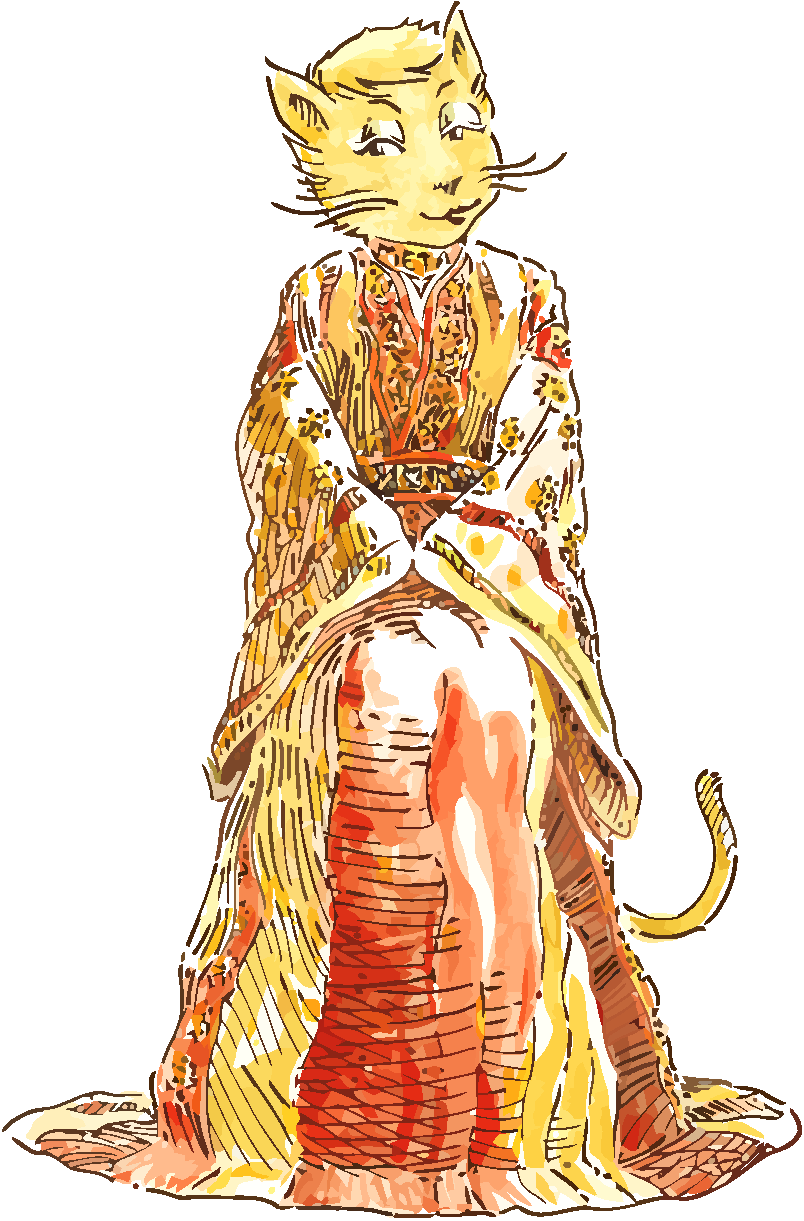
\includegraphics[height=3cm]{meta.pdf}}


%%
\begin{document}

\maketitle

%%
\section{Dancing links}

%
\begin{frame}{Dancing links}
  \begin{itemize}
  \item Exact cover 문제 해결 알고리즘에 사용되는 기법
  \item 백트래킹을 효율적으로 구현하는 방법 ($do$, $undo$ 연산)
  \end{itemize}
\end{frame}

%%
\section{Exact cover 문제}

\begin{frame}{Exact cover 문제}
  \[
  A=
  \begin{pmatrix*}
    0&0&1&0&1&0&0\\
    1&0&0&1&0&0&1\\
    0&1&1&0&0&1&0\\
    1&0&0&1&0&1&0\\
    0&1&0&0&0&0&1\\
    0&0&0&1&1&0&1
  \end{pmatrix*}
  \]
\end{frame}

\begin{frame}[fragile]{Exact cover 문제}
  \centering
  \begin{figure}[!htb]
    \begin{minipage}{.6\textwidth}
      \centering
      $\begin{pmatrix*}
        0&0&1&0&1&0&0\\
        1&0&0&1&0&0&1\\
        0&1&1&0&0&1&0\\
        1&0&0&1&0&1&0\\
        0&1&0&0&0&0&1\\
        0&0&0&1&1&0&1
      \end{pmatrix*}$
    \end{minipage}%
    \begin{minipage}{.4\textwidth}
      \centering
\begin{verbatim}
A B C D E F G
C E
A D G
B C F
A D F
B G
D E G
\end{verbatim}
    \end{minipage}
\end{figure}
\end{frame}

\begin{frame}[fragile]{Algorithm X}
  \begingroup\obeylines
  \baselineskip10pt
If $A$ is empty, the problem is solved; terminate successfully.
Otherwise choose a column, $c$ (deterministically).
Choose a row, $r$, such that $A[r,c]=1$ (nondeterministically).
Include $r$ in the partial solution.
For each $j$ such that $A[r,j]=1$,
\qquad delete column $j$ from matrix~$A$;
\qquad for each $i$ such that $A[i,j]=1$,
\qquad\qquad delete row $i$ from matrix~$A$.
Repeat this algorithm recursively on the reduced matrix~$A$.
\endgroup
\end{frame}

%
\begin{frame}{Dancing links}
\centering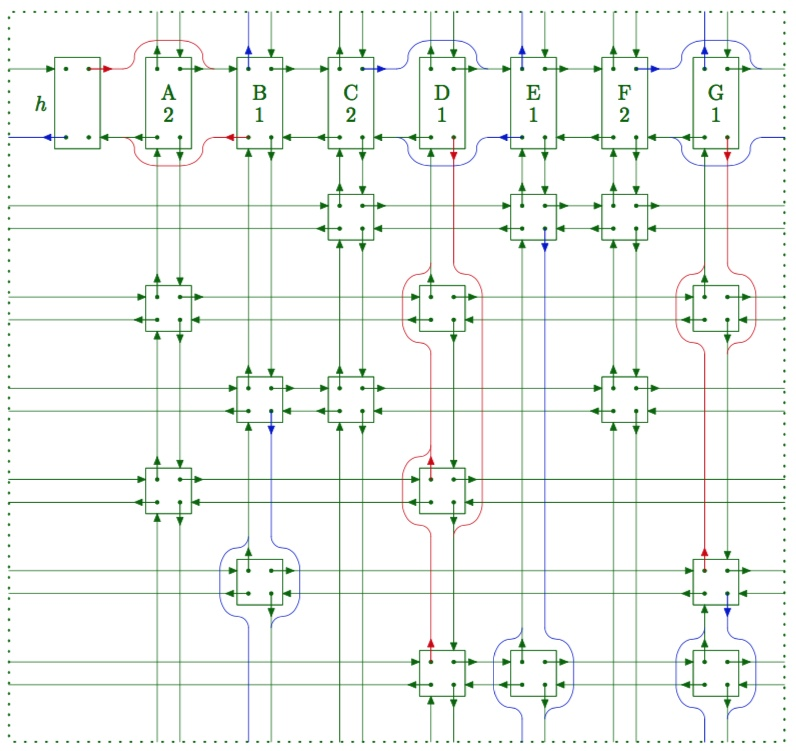
\includegraphics[height=8cm]{dlx.jpg}
\end{frame}

%
\begin{frame}{lua-dancing-links}
\vfill
\begin{center}
\Large
  \href{https://github.com/sjnam/lua-dancing-links}
    {github.com/sjnam/lua-dancing-links}
\end{center}
\vfill
\end{frame}

%%
\section{Polyominoes}

%
\begin{frame}{Pentominoes}
\centering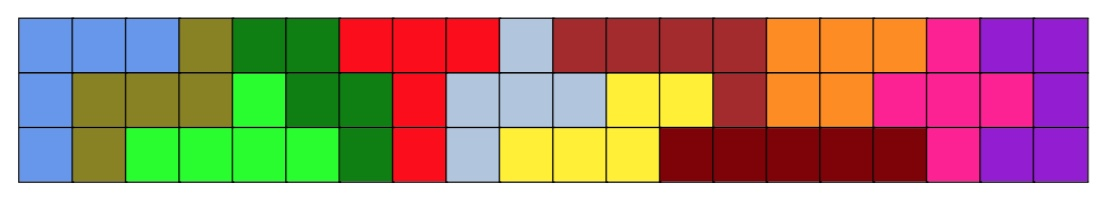
\includegraphics[height=2cm]{3x20.jpg}
\vspace{10mm}
\mbox{\hskip-1cm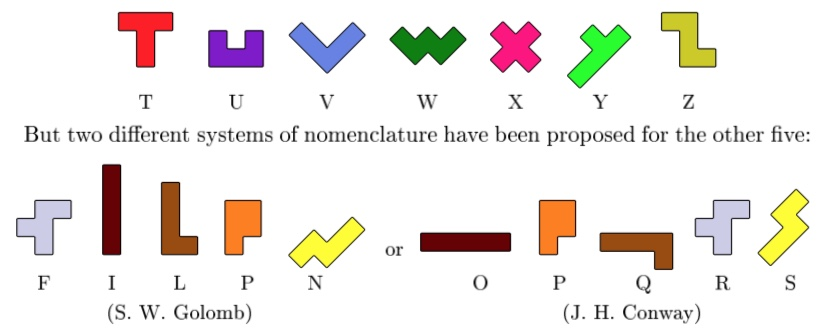
\includegraphics[height=5cm]{pentominoes.jpg}}
\end{frame}

%
\begin{frame}[fragile]{Pentominoes $3\times20$}
\begin{verbatim}
\usepackage{pentominoes}
\pentominoes{3x20.dlx}{3}{20}{5}
\end{verbatim}  
\end{frame}

%%
\section{수도쿠}

%
\begin{frame}[fragile]{수도쿠}
\begin{verbatim}
\usepackage{sudoku-dlx}
\Sudoku{9.......6.3.4....9...915.8..8.5..7..%
..3.9.4....2..1.9.32176....6..1.2.3.8...5...1}
\end{verbatim}  

\begin{center}
  \Sudoku{9.......6.3.4....9...915.8..8.5..7....3.9.4....2..1.9.32176....6..1.2.3.8...5...1}
\end{center}
\end{frame}

%
\begin{frame}[fragile]{수도쿠}
\begin{verbatim}
\Sudoku*{9.......6.3.4....9...915.8..8.5..7..%
..3.9.4....2..1.9.32176....6..1.2.3.8...5...1}
\end{verbatim}

\begin{center}
  \Sudoku*{9.......6.3.4....9...915.8..8.5..7....3.9.4....2..1.9.32176....6..1.2.3.8...5...1}
\end{center}
\end{frame}

%%
\section{$N$ Queens puzzle}

%
\begin{frame}[fragile]{queens}
\begin{verbatim}
\usepackage{queens}
\queens{8}{2}
\end{verbatim}
\vspace{-10mm}
\queens{8}{2}
\end{frame}

%
\begin{frame}{참고}
  \begin{itemize}
  \item \href{http://www-cs-faculty.stanford.edu/~knuth/fasc5c.ps.gz}
    {The Art of Computer Programming PRE-FASCICLE 5C}
  \item \href{https://github.com/sjnam/lua-dancing-links}
    {github.com/sjnam/lua-dancing-links}
  \end{itemize}
\end{frame}


%
\begin{frame}[standout]
  감사합니다
\end{frame}

\end{document}

